\documentclass[a4paper,10pt]{article}

% IMPORTS
\usepackage{amsfonts}
\usepackage{amsmath}
\usepackage{amssymb}
\usepackage{graphicx}
\usepackage{titlesec}
\usepackage{wrapfig}
\usepackage[ngerman]{babel}
\usepackage[utf8x]{inputenc}
\usepackage{pdfpages}
\usepackage{placeins}
\usepackage{color}
\usepackage{eurosym}
\usepackage{xargs}
\usepackage{xcolor}
\usepackage{subcaption}
\usepackage{hyperref}
\usepackage[margin=2cm]{geometry}
\usepackage[colorinlistoftodos,prependcaption,textsize=tiny]{todonotes}

% CONFIG
\clubpenalty = 9000
\widowpenalty = 9000
\displaywidowpenalty = 9000
\titlespacing\section{0pt}{14pt plus 4pt minus 2pt}{2pt plus 2pt minus 1pt}
\titlespacing\subsection{0pt}{10pt plus 4pt minus 2pt}{2pt plus 2pt minus 1pt}
\setlength{\parindent}{0pt}
\setlength{\parskip}{0.5em}
\setcounter{tocdepth}{2}
\newcommand{\cell}[2][c]{\begin{tabular}[#1]{@{}l@{}}#2\end{tabular}}
\renewcommand*\arraystretch{1.3}

% -----------------------------------------------------------------------------
\begin{document}

\begin{flushright}
    Niko Fink\\
    Fabian Knorr
\end{flushright}
\vspace*{-5.5em}

\section*{Aufgabe 5}
\section*{Aufgabe 5b)}

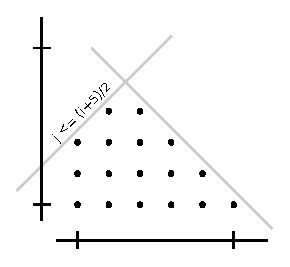
\includegraphics{Polyeder.eps}

$S[i,j]\rightarrow S[i+1,j+1]$

$S[i,j]\rightarrow S[i+3,j+3]$ (ist in der transitiven Hülle der ersten Beziehung enthalten und kann deshalb gestrichen werden)

\texttt{domain = Set("[n] -> \{ S[i,j] : 0 <= i <= n and 0 <= j <= min(n-i, (n+i)/2) \}").coalesce()}

\texttt{Set.coalesce()} vereinfacht Constraints

\texttt{schedule = Map("\{ S[i,j] -> [i,j] \}")}

Ausgabe vom Codegen \texttt{codegen(domain, schedule)} enspricht genau dem Schleifensatz in der Aufgabenstellung.




\end{document}
